\subsection{Machine Learning}
\label{sec:ML}

Machine learning (ML) is a subfield of artificial intelligence (AI), and are methods enabling a computer to improve its performance through experience. Currently, machine learning is one of the top trending technologies, but while machine learning gets increasing attention and interest in today's society, machine learning as a field is not new. Several scientists such as Thomas Ross and Alan Turing did substantial work on building machines that were able learn, and in 1959, Arthur Samuel defines the term machine learning as a \emph{"Field of study that gives computers the ability to learn without being explicitly programmed"}, \citep{ML_def}. Later on Tom M. Mitchell defined learning as \emph{"A computer program is said to \textbf{learn} from experience E with respect to some class of tasks T and performance measure P, if its performance at tasks in T, as measured by P, improves with experience E."}, \citep{Mitchell}.
\nomenclature{AI}{Artificial Intelligence}
\nomenclature{ML}{Machine Learning}

One usually characterize machine learning method based on the learning strategy. The main machine learning categories is broadly classified into supervised, unsupervised and reinforcement learning, as seen in figure \ref{fig:ML_kategorier}. In supervised learning, the model is trained on paired data, with both input and output, in order to predict future events. In unsupervised learning, the model is trained on unlabeled data with no guidance. In this way, the model is looking for hidden patterns in the given data. Reinforcement learning is based on a series of feedback/reward cycles, and learns by interacting with its environment, \citep{Definitions}

\begin{figure}[h!]
\centering
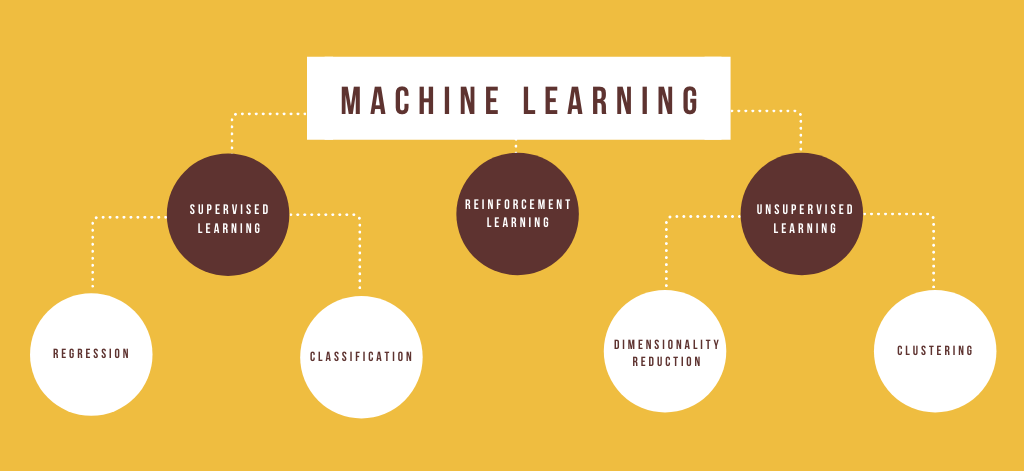
\includegraphics[scale=0.45]{Images/1_introduction/ML_kategorier.png}
\caption{Machine learning categories}
\label{fig:ML_kategorier}
\end{figure}

During the project, supervised learning will be implemented. Supervised learning trains on classified data in order to create a mapping function that can predict future events. The classified data in supervised learning is called a \textbf{training set}, and consists of several \textbf{training examples}. Each training example ($x^{(i)}$,$y^{(i)}$) consists of one \textbf{feature} or input variable, \emph{$x^{(i)}$}, and one \textbf{target} or output variable, \emph{$y^{(i)}$}. Through training on the training set, one wish to learn a function $h : X \mapsto Y$. \emph{h} is commonly known as a \textbf{hypothesis}, and is regarded good if it is able to accurately predict future values of \emph{y}, \citep{Supervised}. A process flow diagram of supervised learning can be seen in figure \ref{fig:supervised}.
\nomenclature{\emph{h}}{Hypothesis}
\nomenclature{\emph{$x^{(i)}$}}{Input variable}
\nomenclature{\emph{$y^{(i)}$}}{Output variable}

\begin{figure}[h!]
\centering
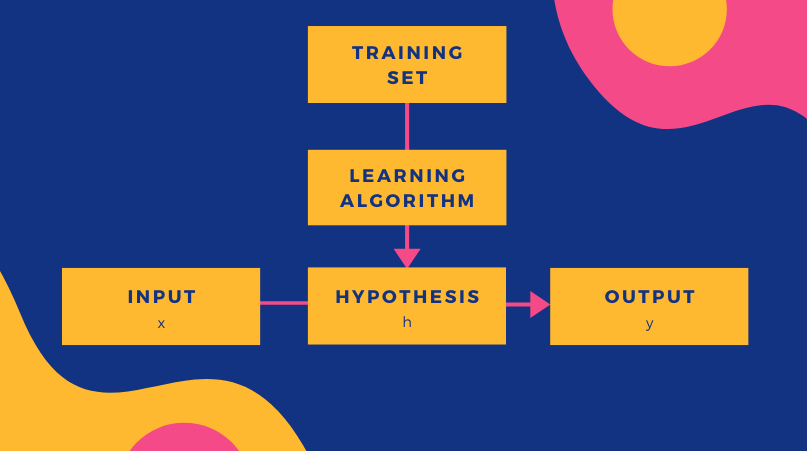
\includegraphics[scale=0.5]{Images/1_introduction/SUPERVISED LEARNING.png}
\caption{Supervised learning process}
\label{fig:supervised}
\end{figure}

Supervised learning is generally classified into two categories; regression and classification. Regression and classification are powerful methods that enables the user to classify and and process data using machine language, and are widely used in industries  such as medicine and finance, \citep{SupMet}. With increased computing powers, these and other machine learning methods will be applicable as solution methods to ever more technological challenges.  

%\todo[inline, color=lightgray!40]
%{
%    Give an overview of machine learning and contextualize it within the overall taxonomy of the field. Introduce supervised learning and some of its methods.
    
%    \vspace{0.2cm}
%}